\chapter{Science of ice reservoirs}

This chapter provides the methodology used to estimate the ice volume evolution and water-use efficiency of
AIRs. The equations governing the mass and energy balance of vertical AIRs (or Icestupas) is explained along
with the associated datasets required for forcing, calibration and validation of this AIR model.

\section{Measurement methodology}

The influence of the chosen location and fountain used was quantified by feeding weather and fountain data to an
energy balance model and validating the ice volume estimates produced with volume observations from drone
flights. Therefore, weather observations and fountain characteristics were required to force the AIR model and
ice volume observations were required to calibrate and validate the model. 

\subsection{Meteorological data}

Air temperature, relative humidity, wind speed, pressure, longwave and global shortwave radiation are required
to calculate the surface energy balance of an AIR. The study period starts when the fountain was forst switched
on and ends when the respective AIR melted completely. These two dates are denoted as start and expiry dates
henceforth. Each AIR is abbreviated based on the country code of the study site with the year of its expiry
date.

\subsection{Fountain observations}

The fountain consists of a pipeline and a nozzle. The pipeline has three attributes, namely : discharge rate
($Q$), height ($h$) and water temperature ($T_F$). Discharge rate represents the discharge rate of the water in
the fountain pipeline. Height denotes the height of the fountain pipeline installed. Fountain water temperature
is the temperature of water droplets produced by the fountain.

The fountain nozzle has three characteristics, namely : the aperture diameter ($dia$), the spray radius ($r$)
and pressure loss ($P$) . Spray radius denotes the observed ice radius formed from the fountain water droplets.
Pressure loss denotes the loss of water head caused due to the fountain nozzle.

\subsection{Drone flights}

\subsection{Study sites}

We chose two villages in the Swiss Alps and the Indian Himalayas called Guttannen and Gangles to collect the
required datasets described above. These two locations exhibit drastically different weather patterns (see
Table) owing to their latitude, longitude and altitude differences. This enabled us to highlight the
meteorological influences on ice volume evolution (RQ 1).

The Guttannen site (46.66 $\degree$N, 8.29 $\degree$E) is situated in the Berne region, Switzerland and has an
altitude of 1047 $m$ a.s.l. In the winter (Oct-Apr), mean daily minimum and maximum air temperatures vary
between -13 and 15 $\degree C$. Clear skies are rare, averaging around 7 days during winter. Daily winter
precipitation can sometimes be as high as 100 $mm$. These values are based on 30 years of hourly historical
weather data measurements \citep{meteoblueClimateGuttannen2021}. Several AIRs were constructed by the Guttannen
Bewegt Association, the University of Fribourg and the Lucerne University of Applied Sciences and Arts during
the winters of 2020-22.

The Gangles site (34.22 $\degree$N, 77.61 $\degree$E) is located around 20 km north of Leh city in the Ladakh
region, lying at 4025 $m$ a.s.l.. The mean annual temperature is $5.6 \, \degree C$, and the thermal range is
characterized by high seasonal variation. During January, the coldest month, the mean temperature drops to $-7.2
\, \degree C$. During August, the warmest month, the mean temperature rises to $17.5 \, \degree C$
\citep{nusserIrrigationDevelopmentUpper2012}. Because of the rain shadow effect of the Himalayan Range, the mean annual precipitation in
Leh totals less than 100 $mm$, and there is high interannual variability. Whereas the average summer rainfall
between July and September reaches 37.5 $mm$, the average winter precipitation between January and March amounts
to 27.3 $ mm$ and falls almost entirely as snow. AIRs were constructed here as part of the Ice Stupa Competition
by the Himalayan Institute of Alternatives, Ladakh (HIAL). 

\section{Modelling methodology}

A bulk energy and mass balance model is used to calculate the amounts of ice, meltwater, water vapour and
wastewater of the AIR. In each hourly time step, the model uses the AIR surface area, energy balance and mass
balance calculations to estimate its ice volume, surface temperature and wastewater as shown in Fig.
\ref{fig:schema} .

\begin{figure}
	\begin{center}
		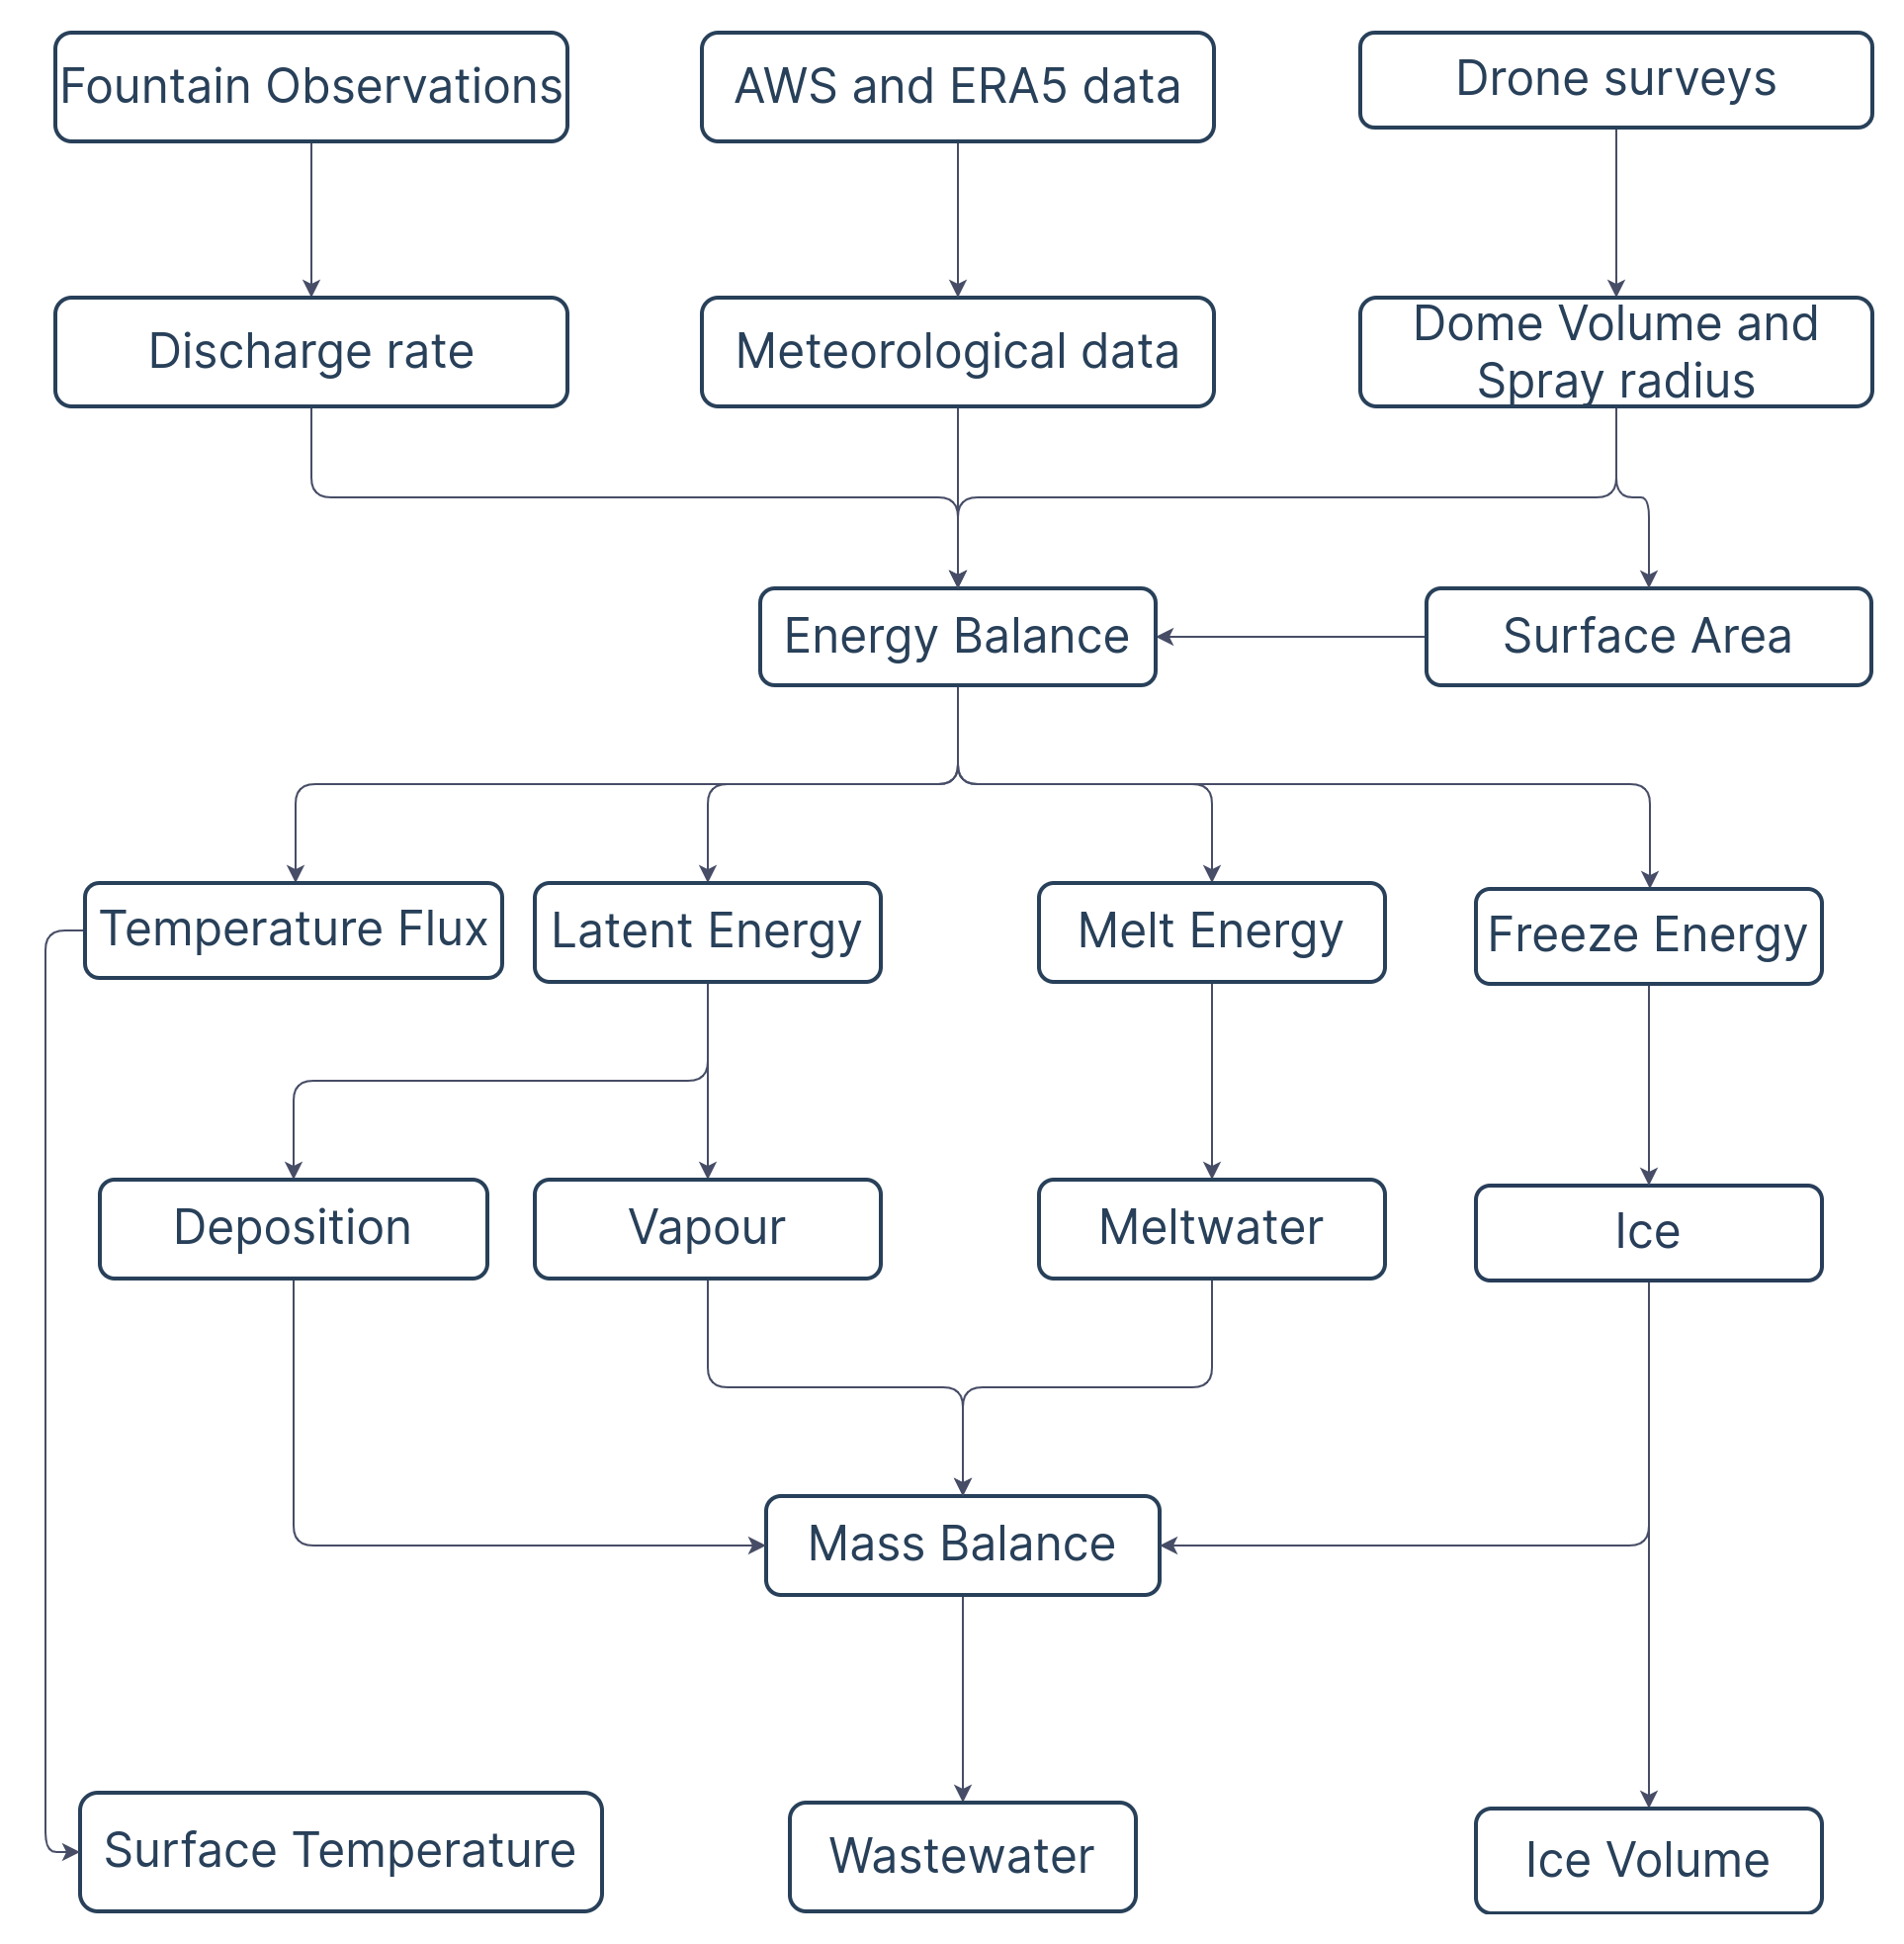
\includegraphics[width=10 cm]{Figures/Figure_3.jpg}
	\end{center}
	\caption{Model schematic showing the workflow used in the model at every time step. }
	\label{fig:schema}
\end{figure}

\subsection{Surface area calculation} \label{sec:shape}

The model assumes the AIR shape to be a cone and assigns the following shape attributes:

\begin{subequations}

	\begin{align}
		\label{eq:A}
		A_{cone}^i & = \pi \cdot r_{cone}^i \cdot \sqrt{{(r_{cone}^i)}^2 + {(h_{cone}^i})^ 2} \\
		\label{eq:V}
		V_{cone}^i & = \pi/3 \cdot {(r_{cone}^i)}^2 \cdot h_{cone}^i                                         \\
		\label{eq:thickness}
		j_{cone}^i & =\frac{\Delta M_{ice}^i}{\rho_{water}* A_{cone}^i}
	\end{align}
\end{subequations}

where $i$ denotes the model time step, $r_{cone}^i$ is the radius; $h_{cone}^i$ is the height; $A_{cone}^i$ is
the surface area; $V_{cone}^i$ is the volume and $j_{cone}^i$ is the AIR surface normal thickness change as shown
in Fig. \ref{fig:shape}. $M_{ice}^i$ is the mass of the AIR and $\Delta M_{ice}^i = M_{ice}^{i-1} -
M_{ice}^{i-2}$. Henceforth, the equations used display the model time step superscript $i$ only if it is different
from the current time step.

AIR density can be defined as:

\begin{equation}
  \rho_{cone} = \frac{M_{F} + M_{dep} + M_{ppt}}{(M_{F} + M_{dep})/\rho_{ice} + M_{ppt}/\rho_{snow}}
\end{equation}

where $M_F$ is the cumulative mass of the fountain discharge; $M_{ppt}$ is the cumulative precipitation;
$M_{dep}$ is the cumulative accumulation through water vapour deposition; $\rho_{ice}$ is the ice density (917
$kg\,m^{-3}$) and $\rho_{snow}$ is the density of wet snow (300 $kg\,m^{-3}$) taken from
\cite{cuffeyPhysicsGlaciers2010} .

AIR volume can also be expressed as:

\begin{equation} V_{cone} =\frac{M_{ice}} {\rho_{cone}} \label{eq:V1} \end{equation}

The initial radius of the AIR is assumed to be $r_F$. The initial height $h_0$ depends on the dome volume
$V_{dome}$ used to construct the AIR as follows:

\begin{equation}
	h_{0} =  \Delta x + \frac{3 \cdot V_{dome}}{\pi \cdot (r_F)^2 }
	\label{eq:h0}
\end{equation}

where $\Delta x$ is the surface layer thickness (defined in Section \ref{sec:energy})

During the subsequent time steps, the dimensions of the AIR evolve assuming a uniform thickness change ($j_{cone}$)
across its surface area with an invariant slope $s_{cone} = \frac{h_{cone}}{r_{cone}}$ .  During these time
steps, the volume is parameterised using Eqn. \ref{eq:V} as:

\begin{equation} V_{cone} = \frac{\pi \cdot {(r_{cone})}^3
		\cdot s_{cone}}{3} \label{eq:V2} \end{equation}

We define the Icestupa boundary through its spray radius, i.e. we assume ice formation is negligible when $r_{cone} >
	r_{F}$. Combining Eqns. \ref{eq:V},  \ref{eq:V1}, \ref{eq:h0} and \ref{eq:V2}, the geometric evolution of the
Icestupa at each time step $i$ can be determined by considering the following rules:

\begin{equation} (r_{cone},\, h_{cone}) = \left\{ \begin{array}{ll} (r_F ,\, h_0)                                                                          & \textit{ if } i=0 \\
		(r_{cone}^{i-1},\, \frac{3 \cdot M_{ice}}{\pi \cdot \rho_{ice} \cdot {(r_{cone}^{i-1})}^2}) & \textit{ if }
		r_{cone}^{i-1} \geq r_{F} \textit{ and } \Delta M_{ice} > 0                                                     \\ (\frac{3 \cdot M_{ice}}{\pi \cdot \rho_{ice} \cdot s_{cone}})^{1/3} \cdot (1,\,  s_{cone}) &
		otherwise\end{array} \right.  \label{eq:A2} \end{equation}



\subsection{Energy balance calculation} \label{sec:energy}

\begin{figure}
	\begin{center}
		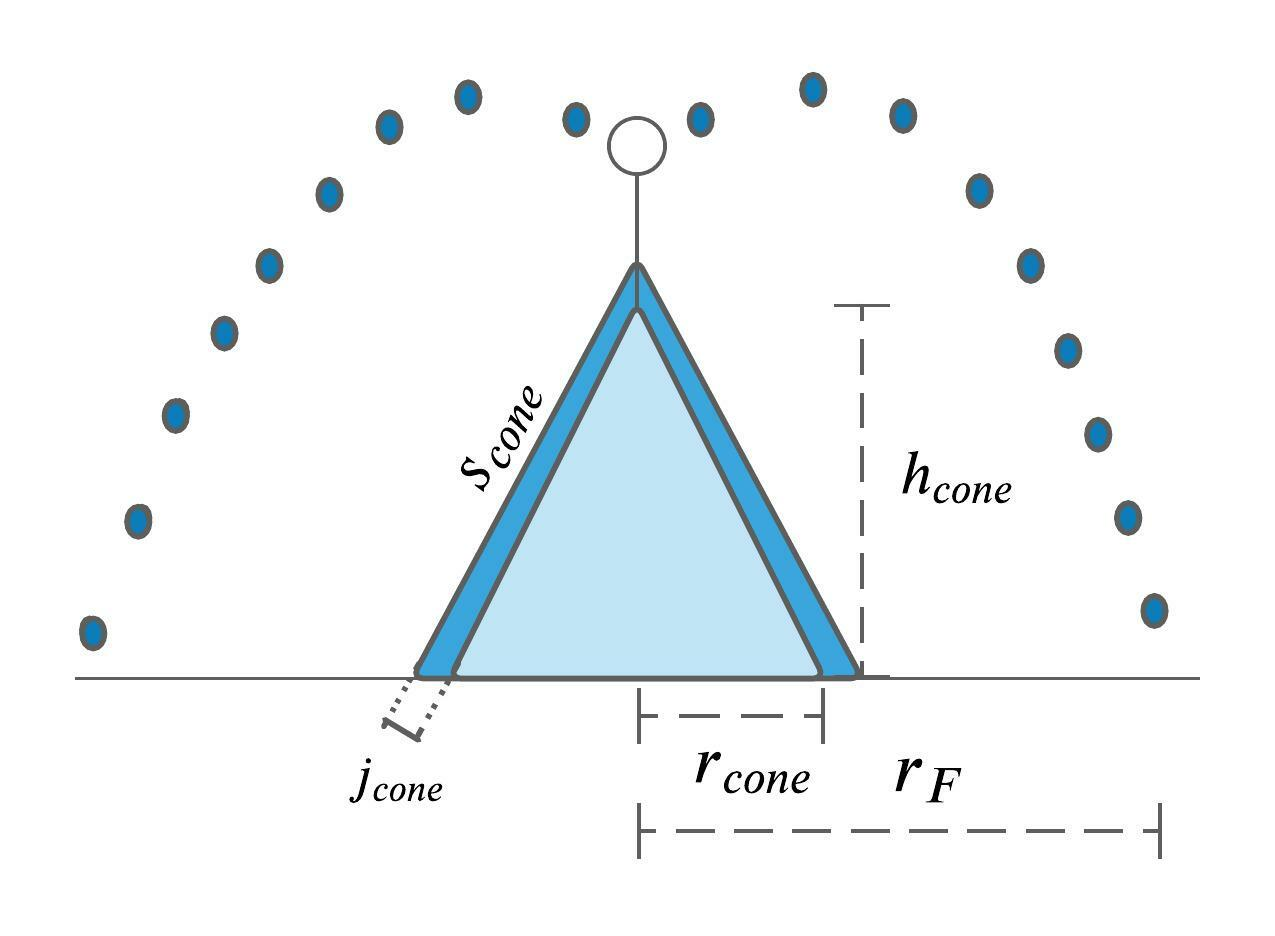
\includegraphics[width=10 cm]{Figures/Figure_4.jpeg}
	\end{center}
	\caption{Shape variables of the AIR. $r_{cone}$ is the radius, $h_{cone}$ is the height, $j_{cone}$ is the
		thickness change and $s_{cone}$ is the slope of the ice cone. $r_F$ is the spray radius of the fountain.}
	\label{fig:shape}
\end{figure}

We approximate the energy balance at the surface of an AIR by a one-dimensional description of energy fluxes
into and out of a (thin) layer with thickness $\Delta x$:

\begin{equation}
	\rho_{ice} \cdot c_{ice} \cdot \frac{\Delta T}{\Delta t} \cdot \Delta x = q_{SW} + q_{LW} + q_{L} + q_{S} + q_{F}+ q_{R} + q_{G}
	\label{eqn:EB}
\end{equation}

Upward and downward fluxes relative to the ice surface are positive and negative, respectively. The first term
is the energy change of the surface layer, which can be translated into a phase change energy should phase
changes occur; $q_{SW}$ is the net shortwave radiation; $q_{LW}$ is the net longwave radiation; $q_{L}$ and
$q_{S}$ are the turbulent latent and sensible heat fluxes. $q_{F}$ and $q_{R}$ represent the heat exchange of
the fountain water droplets and rain droplets with the AIR ice surface respectively. $q_{G}$ represents ground
heat flux between the AIR surface and its interior.

The energy flux acts upon the AIR surface layer, which has an upper and lower boundary defined by the
atmosphere and the ice body of the AIR, respectively.  A sensitivity analysis was later performed
to understand the influence of this factor and decide its value. Here, we define the surface temperature
$T_{ice}$ to be the modelled average temperature of the icestupa surface layer.

\subsubsection{Net Shortwave Radiation \texorpdfstring{$q_{SW}$}{Lg}} \label{sec:SW}

The net shortwave radiation $q_{SW}$ is computed as follows:

\begin{equation} q_{SW} = (1- \alpha)\cdot (SW_{direct} \cdot f_{cone} + SW_{diffuse}) \label{eqn:SW} \end{equation}

where $SW_{direct}$ and $SW_{diffuse}$ are the direct and diffuse shortwave radiation, $\alpha$ is the
modelled albedo and $f_{cone}$ is the area fraction of the ice structure exposed to the direct shortwave
radiation.

The albedo varies depending on the water source that formed the current AIR surface layer. During the fountain
runtime, the albedo assumes a constant value corresponding to ice albedo. However, after the fountain is
switched off, the albedo can reset to snow albedo during snowfall events and then decay back to ice albedo. We
use the scheme described in \cite{oerlemansYearRecordGlobal1998} to model this process. The scheme records the
decay of albedo with time after fresh snow is deposited on the surface. $\delta t$ records the number of time
steps after the last snowfall event. After snowfall, albedo changes over a time step, $\delta t$ , as

\begin{equation} \alpha=\alpha_{ice}+(\alpha_{snow}-\alpha_{ice}) \cdot e^{(-\delta t)/\tau} \label{eqn:a}
\end{equation}

where $\alpha_{ice}$ is the bare ice albedo value (0.25), $\alpha_{snow}$ is the fresh snow albedo value (0.85)
and $\tau$ is a decay rate (16 $days$), which determines how fast the albedo of the ageing snow recedes back to
ice albedo. Discharge events decrease the decay rate by a factor of $\alpha_{ice}/\alpha_{snow}$. 

The solar area fraction $f_{cone}$ of the ice structure exposed to the direct shortwave radiation depends on the shape
considered. Using the solar elevation angle $\theta_{sun}$, the solar beam can be considered to have a vertical
component, impinging on the horizontal surface (semicircular base of the AIR), and a horizontal component
impinging on the vertical cross section (a triangle). The solar elevation angle $\theta_{sun}$ used is modelled
using the parametrisation proposed by \cite{woolfComputationSolarElevation1968}. Accordingly, $f_{cone}$ is determined as follows:

\begin{equation}
	\begin{split}
		f_{cone}& =\frac{(0.5 \cdot r_{cone} \cdot h_{cone}) \cdot cos \theta_{sun} +(\pi \cdot
			{(r_{cone})}^2/2) \cdot sin \theta_{sun} }{\pi \cdot r_{cone} \cdot ({(r_{cone})}^2+{(h_{cone})}^2)^{1/2}}\\
	\end{split}
	\label{eqn:f_{cone} }
\end{equation}

The diffuse shortwave radiation is assumed to impact the conical AIR surface uniformly.

\subsubsection{Net Longwave Radiation \texorpdfstring{$q_{LW}$}{Lg}} \label{sec:LW}

The net longwave radiation $q_{LW}$ is determined as follows:

\begin{equation}
	q_{LW}= LW_{in}-\sigma \cdot \epsilon_{ice} \cdot {(T_{ice}+ 273.15)}^4
	\label{eqn:LW}
\end{equation}

where $T_{ice}$ is the modelled surface temperature given in [$\degree C$],
$\sigma=5.67\cdot10^{-8}\,Jm^{-2}s^{-1}K^{-4}$ is the Stefan-Boltzmann constant, $LW_{in}$ denotes the incoming
longwave radiation and $\epsilon_{ice}$ is the corresponding emissivity value for the Icestupa surface (0.97).

The incoming longwave radiation $LW_{in}$ for the Indian site, where no direct measurements were available, is
determined as follows:

\begin{equation}
	LW_{in}=\sigma \cdot \epsilon_a \cdot {(T_a+ 273.15)}^4
	\label{eqn:LWin}
\end{equation}

here $T_a$ represents the measured air temperature and $\epsilon_a$ denotes the atmospheric emissivity. We
approximate the atmospheric emissivity $\epsilon_a$ using the equation suggested by \cite{brutsaertEvaporationAtmosphereTheory1982},
considering air temperature and vapor pressure (Eqn.  \ref{eqn:atm_e}). The vapor pressure of air over water and
ice was obtained using Eqn. \ref{eqn:vp}.  The expression defined in \cite{brutsaertDerivableFormulaLongwave1975} for clear skies
(first term in equation \ref{eqn:atm_e}) is extended with the correction for cloudy skies after
\cite{brutsaertEvaporationAtmosphereTheory1982} as follows:

\begin{equation}
	\epsilon_a=1.24 \cdot (\frac{p_{v,w}}{(T_a+273.15)})^{1/7}\cdot(1+0.22\cdot{cld}^2) \label{eqn:atm_e}
\end{equation}

with a cloudiness index $cld$, ranging from 0 for clear skies to 1 for complete overcast skies. For the Indian
site, we assume cloudiness to be negligible.

\subsubsection{Turbulent fluxes} \label{sec:Qs}

The turbulent sensible $q_{S}$ and latent heat $q_{L}$ fluxes are computed with the following expressions
proposed by \cite{garrattAtmosphericBoundaryLayer1992}:

\begin{equation}
	q_{S}=\mu_{cone}\cdot c_{a} \cdot \rho_{a} \cdot p_{a}/p_{0,a} \cdot \frac{\kappa^2 \cdot v_a \cdot
		(T_a-T_{ice})}{{(\ln{\frac{h_{AWS}}{z_{0}}})}^2}
	\label{eqn:qs}
\end{equation}

\begin{equation}
	q_{L}=\mu_{cone}\cdot 0.623 \cdot L_s \cdot \rho_{a}/p_{0,a} \cdot \frac{\kappa^2 \cdot
	v_a(p_{v,w}-p_{v,ice})}{{(\ln{\frac{h_{AWS}}{z_{0}}})}^2}
\end{equation}

where $h_{AWS}$ is the measurement height above the ground surface of the AWS (around $2\,m$ for all sites),
$v_a$ is the wind speed in [$m\,s^{-1}$], $c_a$ is the specific heat of air at constant pressure (1010 J
$kg^{-1} K^{-1}$), $\rho_{a}$ is the air density at standard sea level (1.29 $kg m^{-3}$), $p_{0,a}$ is the air
pressure at standard sea level (1013 $hPa$), $p_{a}$ is the measured air pressure, $\kappa$ is the von Karman constant (0.4), $z_{0}$ is the surface
roughness (3 $mm$) and $L_s$ is the heat of sublimation (2848 $kJ\,kg^{-1}$).  The vapor pressure of air with
respect to water ($p_{v,w}$) and with respect to ice ($p_{v,ice}$) was obtained using the formulation given in
\cite{huangSimpleAccurateFormula2018} :

\begin{equation}
	\begin{split}
		p_{v,w}&=e^{\frac{(34.494 - \frac{4924.99}{T_{a} + 237.1})}{(T_a + 105)^{1.57} \cdot 100}} \cdot \frac{RH}{100} \\
		p_{v,ice}&=e^{\frac{(43.494 - \frac{6545.89}{T_{ice} + 278})}{(T_{ice} + 868)^{2} \cdot 100}} \\
	\end{split} \label{eqn:vp}
\end{equation}

The dimensionless parameter $\mu_{cone}$ is an exposure parameter that deals with the fact that AIR has a rough
appearance and forms an obstacle to the wind regime. This factor accounts for the larger turbulent fluxes due to
the roughness of the surface \citep{oerlemansBriefCommunicationGrowth2021}, and is a function of the AIR slope as follows:

\begin{equation}
	\mu_{cone} = 1 + \frac{s_{cone}}{2}
\end{equation}

A possible source of error is the fact that wind measurements from the horizontal plane at the AWS are used,
which might be different from those on a slope. However, without detailed datasets from the AIR surface, we
retain this assumption.

\subsubsection{Fountain discharge heat flux \texorpdfstring{$q_{F}$}{Lg} }

The fountain water, at temperature $T_F$, is assumed to cool to 0 $\degree C$. Thus, the heat flux caused by this
process is:

\begin{equation}
	q_{F} = \frac{ \Delta M_F \cdot c_{water} \cdot T_F}{\Delta t \cdot A_{cone}}
	\label{eqn:qF}
\end{equation}

with $c_{water}$ as the specific heat of water (4186 J $kg^{-1} K^{-1}$).

\subsubsection{Rain heat flux \texorpdfstring{$q_{R}$}{Lg} }

The influence of rain events on the albedo and the energy balance was assumed to be similar to that of discharge
events. However, the water temperature of a ran event was assumed to equal to the air temeperature. Accordingly,
the heat flux generated due to a rain event was equal to:

\begin{equation}
  q_{R} = \frac{ \Delta M_{ppt} \cdot c_{water} \cdot T_a}{\Delta t \cdot A_{cone}}
	\label{eqn:qR}
\end{equation}

\subsubsection{Bulk Icestupa heat flux \texorpdfstring{$q_{G}$}{Lg}} \label{sec:Bulkflux}

The bulk Icestupa heat flux $q_{G}$ corresponds to the ground heat flux in normal soils and is caused by the
temperature gradient between the surface layer ($T_{ice}$) and the ice body ($T_{bulk}$). It is expressed by
using the heat conduction equation as follows:

\begin{equation} q_{G} = k_{ice} \cdot (T_{bulk}-T_{ice}^{i-1})/l_{cone} \label{eqn:qG}    \end{equation}

where $k_{ice}$ is the thermal conductivity of ice (2.123 $W\, m^{-1}\,K^{-1}$) , $T_{bulk}$ is the mean
temperature of the ice body within the icestupa and $l_{cone}$ is the average distance of any point in the
surface to any other point in the ice body. $T_{bulk}$ is initialised as 0 $\degree C$ and later determined from
Eqn. \ref{eqn:qG} as follows:

\begin{equation} T_{bulk}^{i+1} = T_{bulk} - (q_{G} \cdot A \cdot \Delta t)/(M_{ice} \cdot c_{ice}) \end{equation}

Since AIRs typically have conical shapes with $r_{cone} > h_{cone}$, we assume that the center of mass of the cone
body is near the base of the fountain. Thus, the distance of every point in the AIR surface layer from the cone
body's center of mass is between $h_{cone}$ and $r_{cone}$. Therefore, we calculate $q_{G}$ assuming $l_{cone} = (r_{cone} +
	h_{cone})/2$.

\subsubsection{Phase changes}

In this section, the numerical procedures to model phase changes at the surface layer are explained. Let
$T_{temp}$ be the calculated surface temperature. Therefore, Eqn. \ref{eqn:EB} can be rewritten as:

$$q_{total} =\rho_{ice} \cdot c_{ice} \cdot \frac{(T_{temp}-T_{ice})}{\Delta t} \cdot \Delta x$$

where $q_{total}$ represents the total energy available to be redistributed. Even if the numerical heat transfer
solution produces temperatures which are $T_{temp}>0\, \degree C$, say from intense shortwave radiation, the ice
temperature must remain at $T_{temp} = 0\, \degree C$. The ‘‘excess’’ energy is used to drive the melting
process. Moreover, the energy input is used to melt the surface ice layer, and not to raise the surface
temperature to some unphysical value. Similarly, for freezing to occur, three conditions are required. Firstly,
fountain water is present ($\Delta M_{F} > 0 $) and secondly the calculated temperature of the ice, $T_{temp}$,
is below $0\, \degree C$. However, these two conditions are not sufficient as the latent heat turbulent fluxes
can only contribute to temperature fluctuations. Therefore, an additional condition, namely, $(q_{total}-q_{L})
< 0$, is required. Depending on the above conditions, the total energy $q_{total}$ can be redistributed
for the melting ($q_{melt}$), freezing ($q_{freeze}$) and surface temperature change ($q_{T}$) processes as
follows:

\begin{equation}
	q_{total} = \left\{ \begin{array}{ll}
		q_{freeze} + q_{T} & \textit{ if } \Delta M_{F} > 0 \textit{ and } T_{temp} < 0 \textit{ and }(q_{total}-q_{L}) < 0 \\
		q_{melt} + q_{T}   & \textit{ otherwise}
	\end{array} \right.
\end{equation}

Henceforth, time steps when the the total energy is redistributed to the freezing energy are called freezing
events and the rest of the time steps are called melting events.


During a freezing event, the AIR surface is assumed to warm to $0 \degree C$. The available energy
$(q_{total}-q_{L})$ is further increased due to this change in surface temperature represented by the energy
flux:

$$q_{0} = \frac{\rho_{ice} \cdot \Delta x \cdot c_{ice} \cdot T_{ice}^{i-1}}{\Delta t}$$

The available fountain discharge ($\Delta M_{F}$) may not be sufficient to utilize all the freezing energy. At such times, 
the additional freezing energy further cools down the surface temperature. Accordingly, the surface energy flux
distribution during a freezing event can be represented as:

\begin{equation}
	(q_{freeze}, q_{T}) = \left\{ \begin{array}{ll}
		(\frac{\Delta M_{F} \cdot L_f
		}{A_{cone} \cdot \Delta t}
		, q_{total}+\frac{\Delta M_{F} \cdot L_f
		}{A_{cone} \cdot \Delta t})          & \textit{ if  } \Delta M_{F} \textit{ insufficient }\\
		(q_{total}-q_{L}+q_{0}, q_{L}-q_{0}) & \textit{ otherwise }                                                                      \\
	\end{array} \right.
\end{equation}

If $T_{temp} > 0 \degree C$, then energy is reallocated from $q_{T}$ to $q_{melt}$ to maintain surface
temperature at melting point. The total energy flux distribution during a melting event can be represented as:

\begin{equation}
	(q_{melt}, q_{T}) = \left\{ \begin{array}{ll}
		(0, q_{total})
    & \textit{ if } T_{temp} \leq 0 \\
		(\frac{T_{temp} \cdot \rho_{ice} \cdot c_{ice} \cdot \Delta x}{\Delta t}, q_{total}-\frac{T_{temp} \cdot \rho_{ice} \cdot c_{ice} \cdot \Delta x}{\Delta t}  ) & \textit{ if } T_{temp} > 0
	\end{array} \right.
\end{equation}


\subsection{Mass balance calculation}

The mass balance equation for an AIR is represented as:

\begin{equation}
	\frac{\Delta M_{F} + \Delta M_{ppt} + \Delta M_{dep}}{\Delta t} = \frac{\Delta M_{ice} +\Delta M_{water} +
		\Delta M_{sub} + \Delta M_{waste}}{\Delta t}  \\
	\label{eq:MB}
\end{equation}

where $M_{F}$ is the cumulative mass of the fountain discharge; $M_{ppt}$ is the cumulative precipitation;  $M_{dep}$ is the cumulative
accumulation through water vapour deposition; $M_{ice}$ is the cumulative mass of ice; $M_{water}$ is the cumulative
mass of melt water; $M_{sub}$ represents the cumulative water vapor loss by sublimation and $M_{waste}$ represents the
fountain wastewater that did not interact with the AIR. The left hand side of equation \ref{eq:MB} represents the rate of
mass input and the right hand side represents the rate of mass output for an AIR.

Precipitation input is calculated as shown in equation \ref{eq:ppt} where $\rho_{w}$ is the density of water (1000
$kg\,m^{-3}$), $\Delta ppt/ \Delta t$ is the measured precipitation rate in [$m\,s^{-1}$] and $T_{ppt}$ is the temperature threshold
below which precipitation falls as snow. Here, snowfall events were identified using $T_{ppt}$ as $1 \degree C$. Snow
mass input is calculated by assuming a uniform deposition over the entire circular footprint of the AIR.

The latent heat flux is used to estimate either the evaporation and condensation processes or sublimation and deposition
processes as shown in equation \ref{eq:vap}. During the time steps at which the surface temperature is below 0 $\degree C$ only
sublimation and deposition can occur, but if the surface temperature reaches 0 $\degree C$, evaporation and condensation
can also occur. As the differentiation between evaporation and sublimation (and condensation and deposition) when the
air temperature reaches 0 $\degree C$ is challenging, we assume that negative (positive) latent heat fluxes correspond
only to sublimation (deposition), i.e. no evaporation (condensation) is calculated.

Since we have categorized every time step as a freezing or melting event, we can determine the melting/freezing
rates and the corresponding meltwater/ice quantities as shown in equations \ref{eq:m_freeze/melt}, \ref{eq:mwat}
and \ref{eq:mcone}. Having calculated all other mass components, the fountain wastewater generated every
time step can be calculated using Eqn. \ref{eq:MB}.

\begin{subequations}
	\begin{align}
		\frac{\Delta M_{F}}{\Delta t} & = \left\{ \begin{array}{ll} \frac{60}{\rho_w \cdot \Delta t} \cdot d_F
			 & \textit{ if fountain is on} \\ 0 & \textit{ otherwise } \\\end{array} \right.                                             \\
		\label{eq:ppt}
		\frac{\Delta M_{ppt}}{\Delta t}                                    & = \left\{ \begin{array}{ll} \pi \cdot
        {(r_{cone})}^2 \cdot
			\rho_{w}\cdot \frac {\Delta ppt}{\Delta t} & \textit{ if } T_{a} < T_{ppt} \\ 0 & \textit{ if } T_{a} \geq T_{ppt} \\\end{array} \right.                                             \\
		\label{eq:vap}
		(\frac{\Delta M_{dep}}{\Delta t}, \frac{\Delta M_{sub}}{\Delta t}) & = \left\{ \begin{array}{ll} \frac{q_{L}
			\cdot A_{cone}}{L_s}\cdot (1,0)  & \textit{ if } q_{L} \geq 0 \\ \frac{q_{L}
			\cdot A_{cone}}{L_s}\cdot (0,-1) & \textit{ if } q_{L} < 0    \\\end{array} \right.                                             \\
		\label{eq:mwat}
		\frac{\Delta M_{water}}{\Delta t}                                  & = \frac{q_{melt} \cdot A_{cone} }{L_f}                                                   \\
	  \label{eq:m_freeze/melt}
    \frac{\Delta M_{freeze/melt}}{\Delta t} & = \frac{q_{freeze/melt} \cdot A_{cone} }{L_f} \\
		\label{eq:mcone}
		\frac{\Delta M_{ice}}{\Delta t}                                    & = \frac{q_{freeze}\cdot A_{cone} }{L_f} + \frac{\Delta M_{ppt}}{\Delta t} + \frac{\Delta
			M_{dep}}{\Delta t}- \frac{\Delta M_{sub}}{\Delta t}- \frac{\Delta M_{water}}{\Delta t}
	\end{align}
\end{subequations}

Considering AIRs as water reservoirs, their net water loss can be defined as:

\begin{equation} \textit{Net water losses} = \frac{M_{waste}+M_{sub}}{(M_F+M_{ppt}+M_{dep})} \cdot 100 \end{equation}



